%%%%%%%%%%%%%%%%%%%%%%%%%%%%%%%%%%%%%%%%%%%%%%%%%%%%%%%%%%%%%%%%
% %
% Seth Cram %
% ECE351 Section 53 %
% Lab 5 %
% Due 02/22/2022 %
% Any other necessary information needed to navigate the file %
%
%
% %
%%%%%%%%%%%%%%%%%%%%%%%%%%%%%%%%%%%%%%%%%%%%%%%%%%%%%%%%%%%%%%%%
%%%%%%%%%%%%%%%%%%%%%%%%%%%%%%%%%%%%%%%%%%%
%%% DOCUMENT PREAMBLE %%%
\documentclass[12pt]{report}
\usepackage[english]{babel}
%\usepackage{natbib}
\usepackage{url}
\usepackage[utf8x]{inputenc}
\usepackage{amsmath}
\usepackage{graphicx}
\graphicspath{{images/}}
\usepackage{parskip}
\usepackage{fancyhdr}
\usepackage{vmargin}
\usepackage{listings}
\usepackage{hyperref}
\usepackage{xcolor}
\usepackage{verbatim}

\definecolor{codegreen}{rgb}{0,0.6,0}
\definecolor{codegray}{rgb}{0.5,0.5,0.5}
\definecolor{codeblue}{rgb}{0,0,0.95}
\definecolor{backcolour}{rgb}{0.95,0.95,0.92}

\begin{comment} %have to use verbatim package for this

\section{Personal Notes}
            


\end{comment}

\lstdefinestyle{mystyle}{
    backgroundcolor=\color{backcolour},   
    commentstyle=\color{codegreen},
    keywordstyle=\color{codeblue},
    numberstyle=\tiny\color{codegray},
    stringstyle=\color{codegreen},
    basicstyle=\ttfamily\footnotesize,
    breakatwhitespace=false,         
    breaklines=true,                 
    captionpos=b,                    
    keepspaces=true,                 
    numbers=left,                    
    numbersep=5pt,                  
    showspaces=false,                
    showstringspaces=false,
    showtabs=false,                  
    tabsize=2
}
 
\lstset{style=mystyle}

\setmarginsrb{3 cm}{2.5 cm}{3 cm}{2.5 cm}{1 cm}{1.5 cm}{1 cm}{1.5 cm}

\title{Lab 5}		%TITLE						
% Title
\author{ Seth Cram}						
% Author
\date{02/22/2022}
% Date

\makeatletter
\let\thetitle\@title
\let\theauthor\@author
\let\thedate\@date
\makeatother

\pagestyle{fancy}
\fancyhf{}
\rhead{\theauthor}
\lhead{\thetitle}
\cfoot{\thepage}
%%%%%%%%%%%%%%%%%%%%%%%%%%%%%%%%%%%%%%%%%%%%
\begin{document}

%%%%%%%%%%%%%%%%%%%%%%%%%%%%%%%%%%%%%%%%%%%%%%%%%%%%%%%%%%%%%%%%%%%%%%%%%%%%%%%%%%%%%%%%%

\begin{titlepage}
	\centering
    \vspace*{0.5 cm}
   % \includegraphics[scale = 0.075]{bsulogo.png}\\[1.0 cm]	% University Logo
\begin{center}    \textsc{\Large   ECE 351 - 53 }\\[2.0 cm]	\end{center}% University Name
	\textsc{\Large Step and Impulse Response of RLC Band Pass Filter }\\[.5 cm]				% Course Code
	\rule{\linewidth}{0.2 mm} \\[0.4 cm]
	{ \huge \bfseries \thetitle}\\
	\rule{\linewidth}{0.2 mm} \\[1.5 cm]
	
	\begin{minipage}{0.4\textwidth}
		\begin{flushleft} \large
		%	\emph{Submitted To:}\\
		%	Name\\
          % Affiliation\\
           %contact info\\
			\end{flushleft}
			\end{minipage}~
			\begin{minipage}{0.4\textwidth}
            
			\begin{flushright} \large
			\emph{Submitted By :} \\
			Seth Cram  
		\end{flushright}
           
	\end{minipage}\\[2 cm]
	
\end{titlepage}

%%%%%%%%%%%%%%%%%%%%%%%%%%%%%%%%%%%%%%%%%%%%%%%%%%%%%%%%%%%%%%%%%%%%%%%%%%%%%%%%%%%%%%%%%

\tableofcontents
\pagebreak

%%%%%%%%%%%%%%%%%%%%%%%%%%%%%%%%%%%%%%%%%%%%%%%%%%%%%%%%%%%%%%%%%%%%%%%%%%%%%%%%%%%%%%%%%
\renewcommand{\thesection}{\arabic{section}}

\section{Introduction}

The goal of lab 5 is to utilize Laplace transforms to find the time-domain step-response and impulse-response of an RLC bandpass
filter using Python in the Spyder IDE.

\section{Equations}
    \begin{equation*}
        u(t) = \{t<0:0, t>=0:1\}
    \end{equation*}
 
    \begin{equation*}
        u(s) = 1/s
    \end{equation*}
 
    \begin{equation*}
        H(s) = V_{out}(s)/V_{in}(s) = Ls/(Ls + R(1 + LCs^2)
    \end{equation*}
    
     \begin{equation*}
        h(t) = 10,000 \cdot e^{-5000t} \cdot ( cos(18,584t) - 0.269sin(18,584t) )
    \end{equation*}
    
    \begin{equation*}
        H(s) \cdot u(s) = ( Ls/(Ls + R(1 + LCs^2) ) \cdot 1/s \\
                        = L/(Ls + R(1 + LCs^2)
    \end{equation*}

    \begin{equation*}
       [ H(s) \cdot u(s) ]_{s -> 0}: Ls/(Ls + R(1 + LCs^2) \\
                                = 0
    \end{equation*}
    
\section{Methodology}

%This section will describe how you went about solving the lab. Make sure you go into detail about any method you used. %Include coding samples here if necessary. This is also where you would include necessary derivations. An example of %inserting code into the report is given. Do not go overboard on inserting code into your report, only use whats %absolutely necessary to illustrate your point.

    \paragraph{} For lab 5, we were assigned a prelab. For this, we used Laplace transforms to find the time-domain step-response and impulse-response of an RLC bandpass filter. As seen in the Results section, we derived the transfer function, H(s), in terms of R, L and C. Then, proceeded to find the impulse response, h(t). Since the transfer function was a complicated one, I couldn't easily compute the inverse Laplace function of it. So, I used an inverse Laplace function on my calculator to come up with the corresponding time-domain function. 
    
    \paragraph{} Moving onto the actual lab, I began computing the impulse response. I typed in the function I derived during the prelab and graphed that without issue. Using the library impulse function was a bit less intuitive. I'm grateful for the example code provided on the handout that showed how to use it. 
    
    \paragraph{} Graphing the step response was similar to plotting the impulse response, so using the library function was a breeze. Doing the final value theorem calculation for the step response in the Laplace domain was a bit more difficult. Having just been introduced to the material yesterday, I needed a reminder of how it was supposed to work and the general formula. The calculation itself ended up being rather simple, as seen in the Equations section of my report. 
    
\section{Results}

%This section will go over the results of the lab. Use this area to describe %if the lab worked as expected or if the results are unexpected or different %from your hand calculations or intuition. Part of being a good engineer is %gaining intuition about these problems and being able to understand quickly %if something is wrong. Use code, plots, tables, and figures as necessary. %Make sure to cite all other works used and note them in the bibliography. A %sample entry is in this document.

    \paragraph{} Since the transfer function is Vout/Vin, I expected the equivalent equation in terms of R, L and C to be rather complicated and the denominator to hold s-terms.
    
    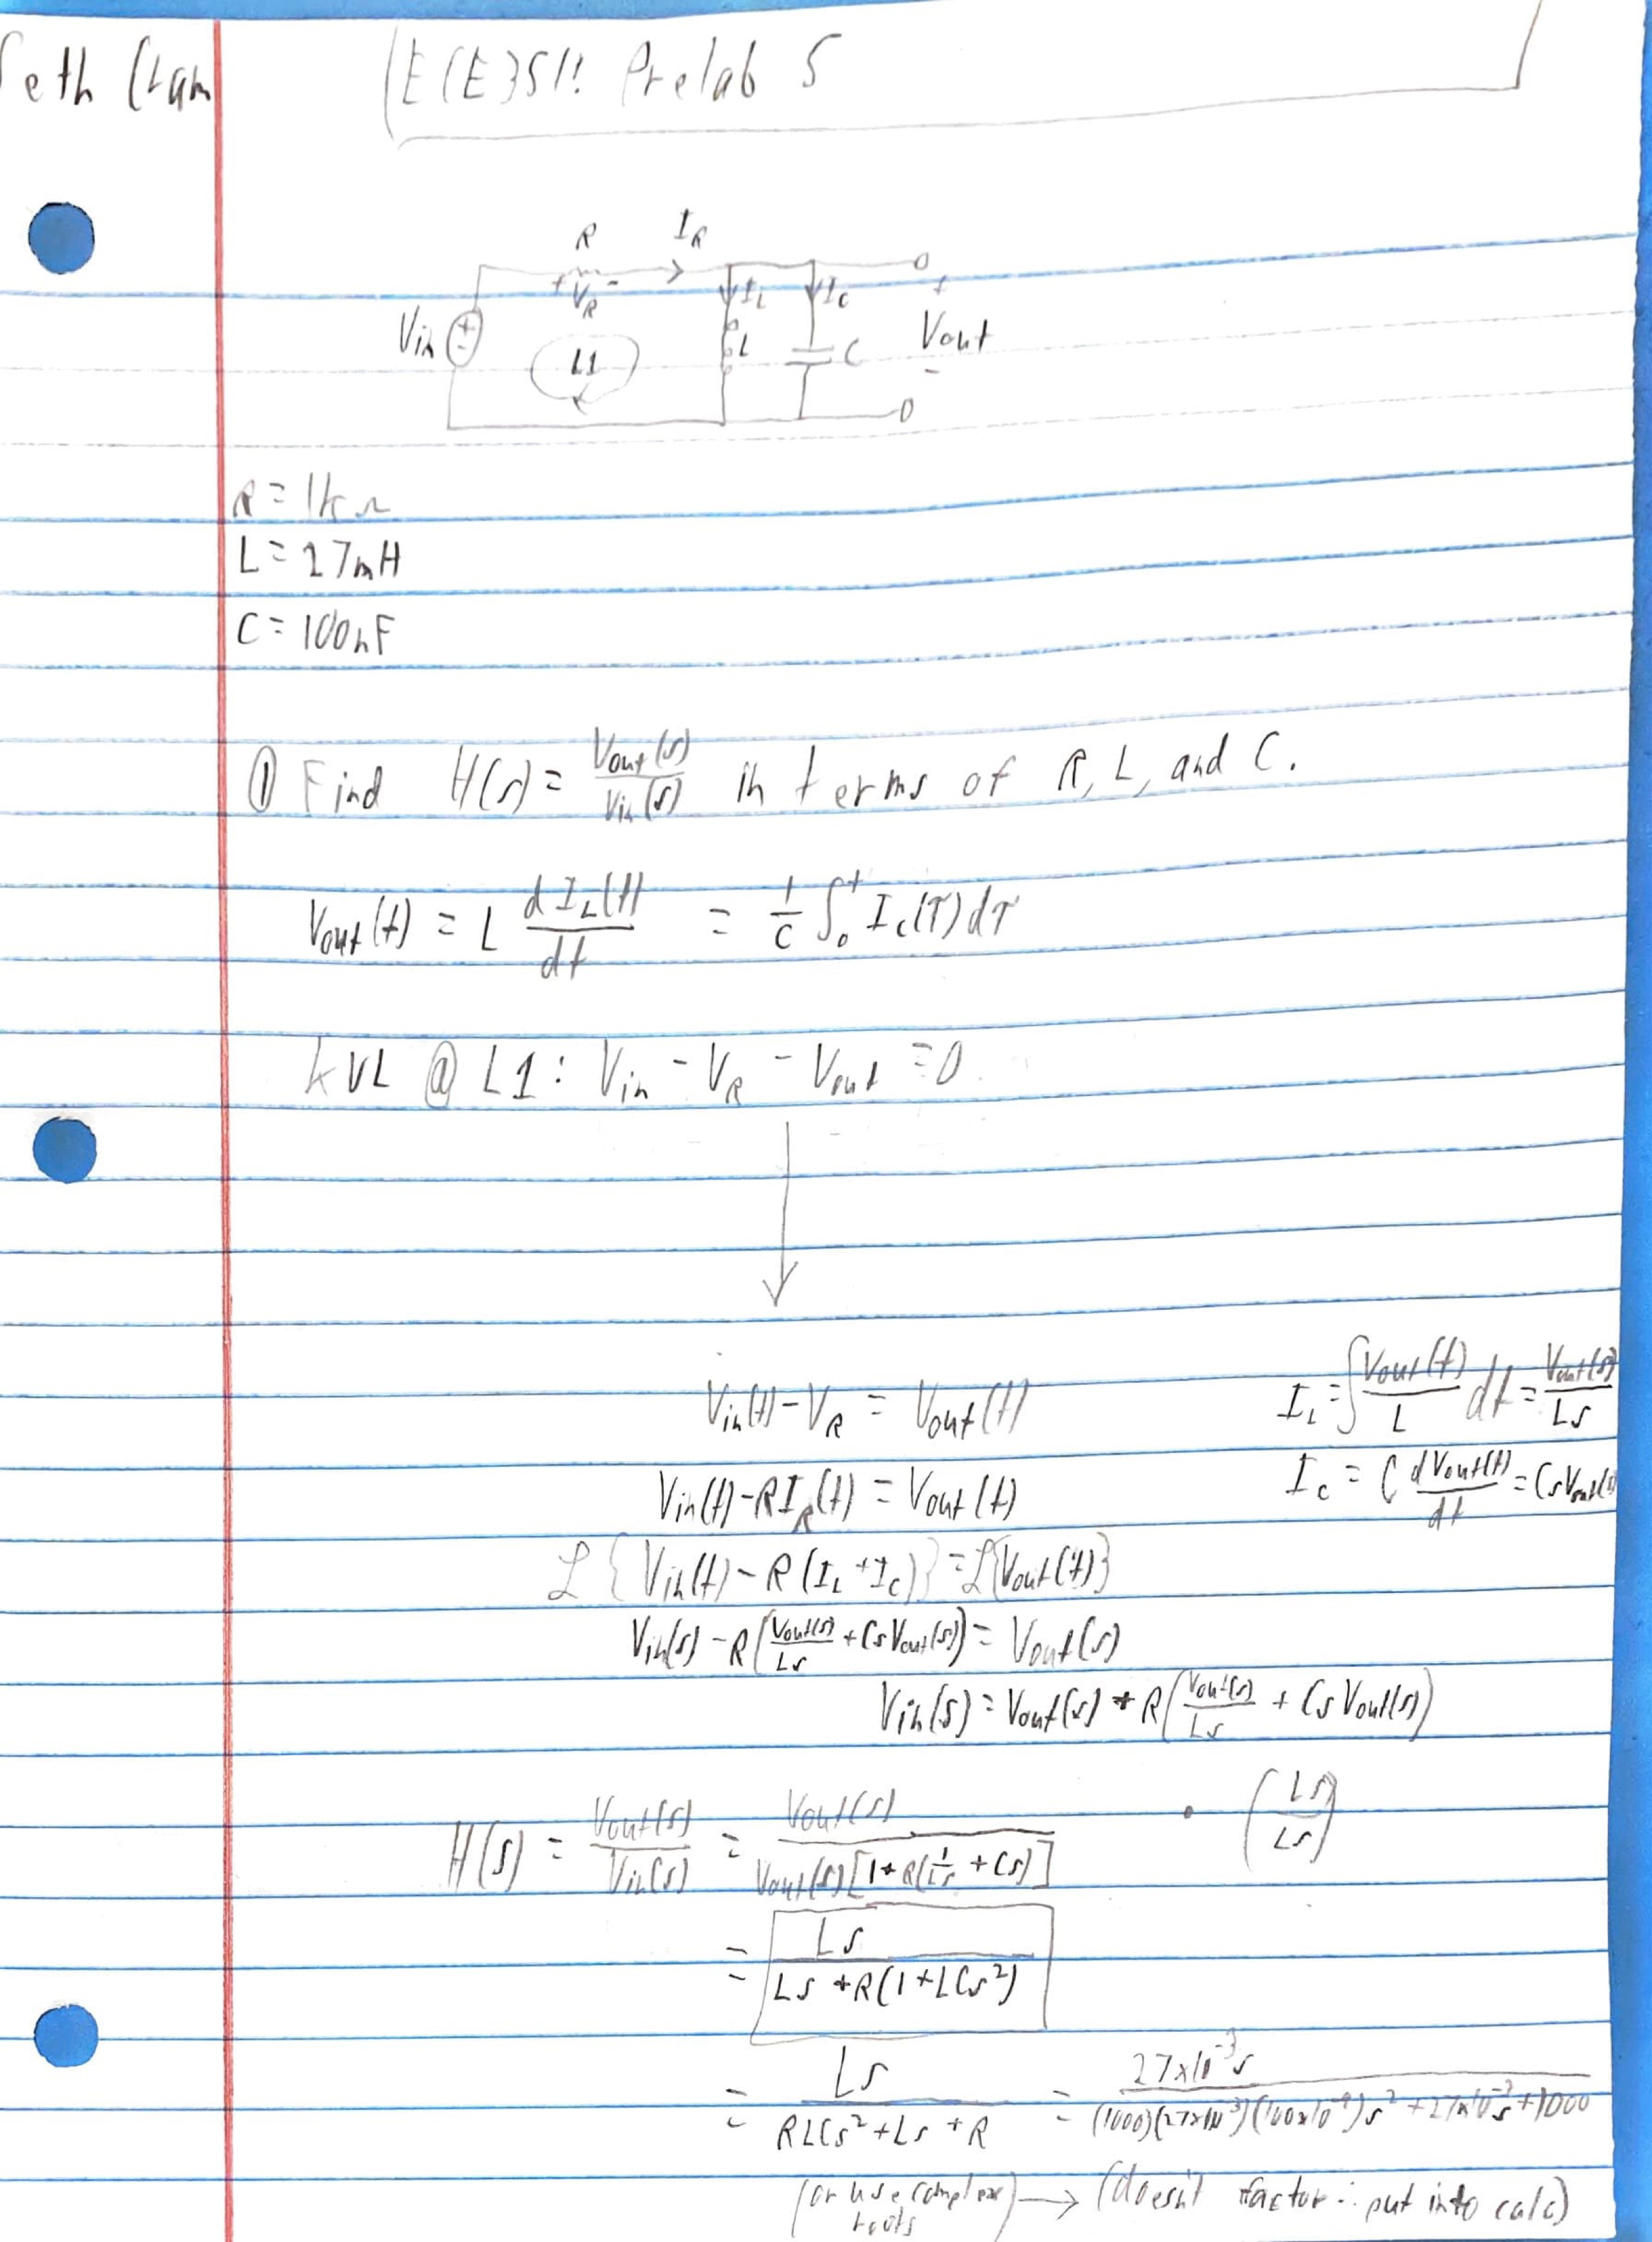
\includegraphics[scale=0.15]{EB56ECFA-E791-46BE-ACBF-A6EA65DBC192.jpeg}
    
    \paragraph{} My expectation partially held true. Although, I didn't predict an s-term in the numerator or multiple s-terms in the denominator. 

    \paragraph{} I expected the impulse response function to be an exponential function because of the s-term in the denominator. 

    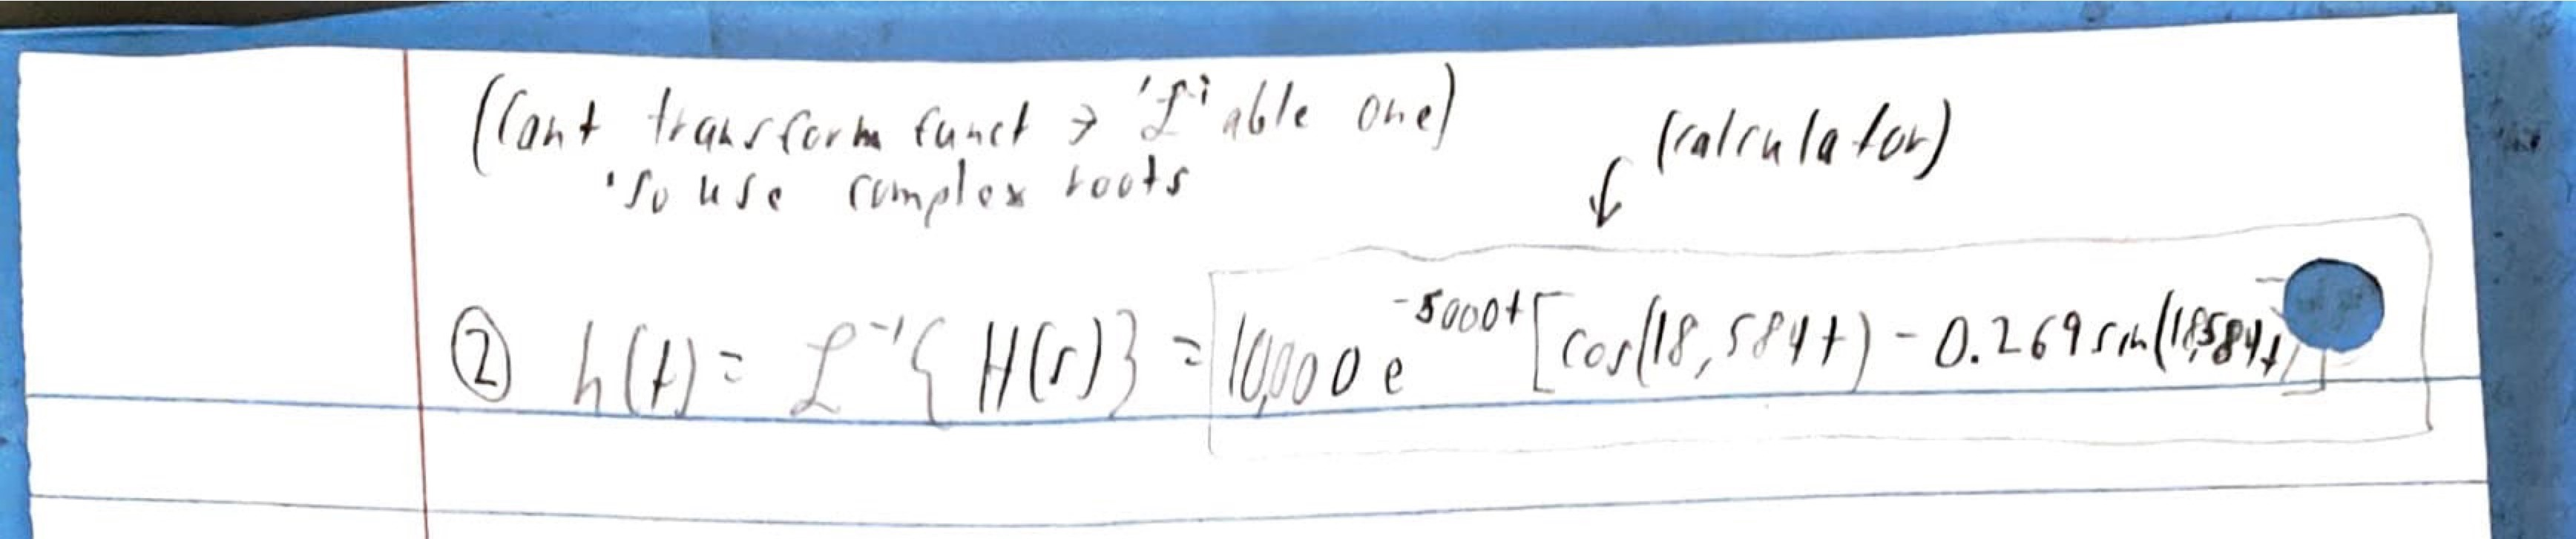
\includegraphics[scale=0.15]{B2D35933-62AD-46D5-A15F-ED4A113534AF.jpeg}

    \paragraph{} I did not expect the impulse response function to be trigonometric functions. Looking back at a Laplace table, it makes sense for at least one trigonometric function to be involved, since they're the only ones with an $s^{2}$ term and arithmetic in the denominator. 
    
    \paragraph{} For the impulse responses, I expected them to approach zero eventually because of the exponential term in the denominator. 
    
    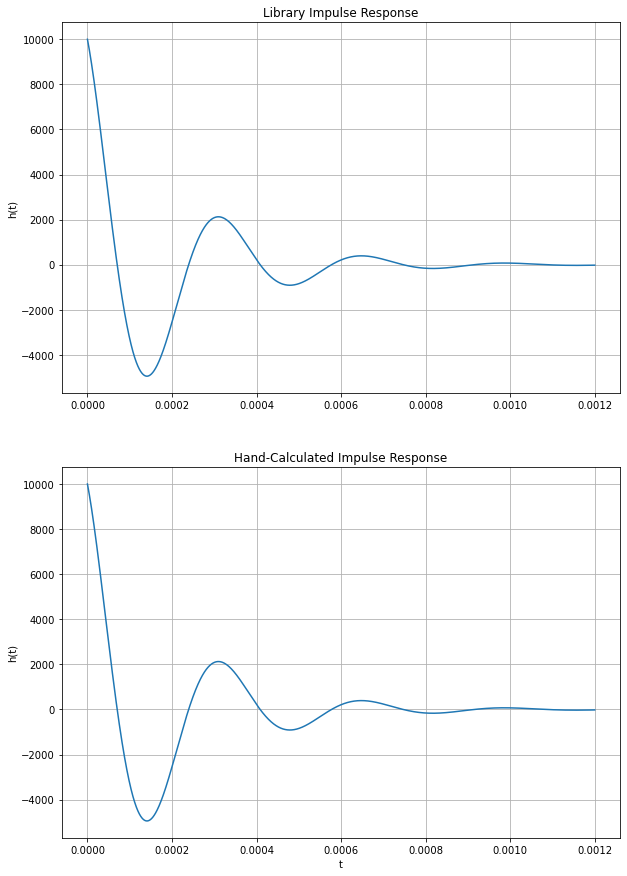
\includegraphics[scale=0.6]{impulse response.png}
    
    \paragraph{} As seen above, my expectation held true, although I didn't foresee such a large range of values being reached toward the beginning. Looking back at the equation, that behavior lines up with the large coefficient in the numerator.
    
    \paragraph{} For the step response, I expected the curve from the first part shifted over to the right because of the step function's involvement. 
    
    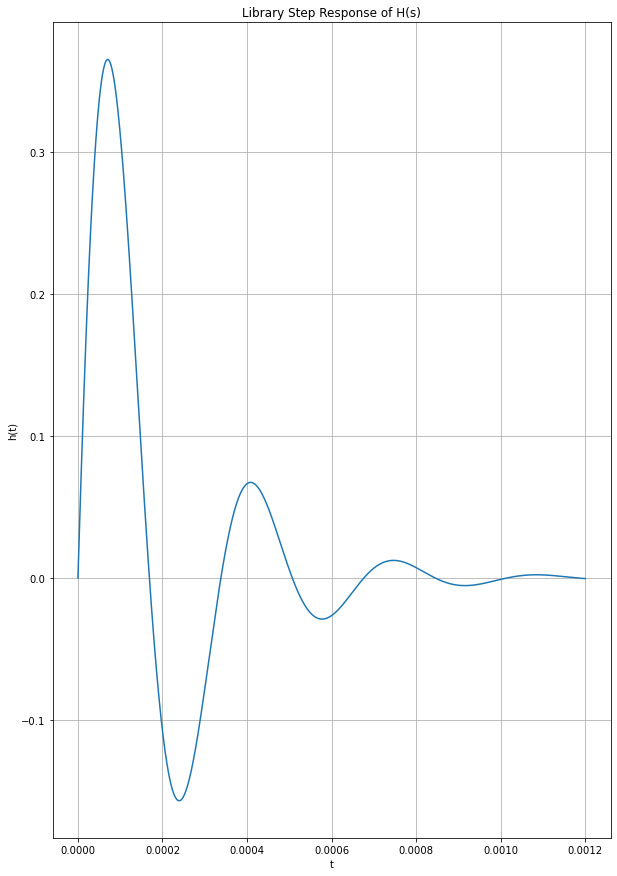
\includegraphics[scale=0.6]{step response.png}
    
    \paragraph{} The shift lines up with my expectations, but I didn't expect to see such a large decrease in the y-scale. Although it keeps roughly the same shape as the impulse response, the y-scales are wildly different. 
      
    \paragraph{} My answer of zero for the final value theorem calculation performed on the step response, makes sense because, as seen in the previous plot, zero is rapidly approached. The main reasoning for such a small time scale is because of this rapid zeroing out. Another reason zero makes sense is because a result of zero means the system is stable. We expect an RLC circuit such as this to be stable. 

\section{Error Analysis}

%This section will discuss error analysis of the experiment. Since this lab %deals with ideal simulation there shouldn't be any sources of error, so %instead this section can be used to describe any difficulties you had during %lab and how you solved them. Alternatively, if you couldn't get the %experiment to work, which is okay, you need to use this section to explain why %you couldn't get it to work to earn full points. 

\paragraph{} A possible source of error could be the approximation when calculating our user-defined impulse function. Approximation tends to trickle down when done early on. 

\paragraph{} The main difficulty I encountered was calculating the impulse response using the sin-method. Initially, I merely plugged it into my calculator and wrote down an answer. But when we learned about the sin-method in-class, I decided to try and give it a go by-hand. I ended up with an incorrect result and wasn't able to determine the source of my error, so I defaulted to my calculator's answer.  

\section{Questions} %also address any deliverables not yet put in yet
    \begin{enumerate}
        \item Explain the result of the Final Value Theorem from Part 2 Task 2 in terms of the physical circuit components.
        \paragraph{} The result of the Final Value Theorum is zero because of how the inductor and capacitor interact in the RLC circuit. Their incremental charging and discharging of current and voltage result in a stable system. As seen when converting a capacitor's current and an inductor's voltage into the s-domain, having these s terms approach zero results in zero for both of these component values. 
        
        \item Leave any feedback on the clarity of lab tasks, expectations, and deliverables
        \paragraph{} The clarity of the prelab, expectations and deliverables was great. 
    \end{enumerate}

\section{Conclusion}

%Discuss briefly what you learned in this lab and whether or not you feel the %lab was successful. Include any recommendations for future labs as this is a %learning experience for all of us. Discuss any insights you gained from this %lab and how that will affect future work. \textit{Note: The bibliograhpy %needs to be on its own page.}

    \paragraph{} During lab 5, I went through the step and impulse response of an RLC Band Pass Filter. In summary, I learned how to use tuples in Python to input to a function and capture output from a function, how to use the final value theorem in a useful manner and what the results of the final value theorem tell us about a system. The lab was successful. Although I didn't use it 100\% correctly, having experience with the sin-method will be useful when dealing with complex roots from now on. 

Github: \url{https://github.com/SethCram} 

\newpage

\end{document}